% Recycling the Living
% Dormant-neuron interventions do not work by reviving dead units.
%
% Built with the official TMLR style file, fetched from
%   https://github.com/JmlrOrg/tmlr-style-file  (linked from https://jmlr.org/tmlr/)
% and used unmodified: tmlr.sty, tmlr.bst, fancyhdr.sty, math_commands.tex.
%
% The [preprint] option de-anonymises the author block. TMLR submissions are
% anonymous -- switch to a bare \usepackage{tmlr} before submitting, and to
% \usepackage[accepted]{tmlr} for a camera-ready version.
%
% Every number in this file is generated by paper/collect_numbers.py, which reads
% the committed parquet outputs in runs/_extracts/ and applies the frozen
% estimator from configs/analysis_plan.json. Nothing is typed in from a prose
% summary. Regenerate with:  python paper/collect_numbers.py

\documentclass[10pt]{article}
\usepackage[preprint]{tmlr}

\usepackage{hyperref}
\usepackage{url}
\usepackage{booktabs}
\usepackage{amsmath}
\usepackage{amssymb}
\usepackage{graphicx}
\usepackage{tikz}
\usetikzlibrary{decorations.pathreplacing, positioning, arrows.meta}
\usepackage{multirow}
\usepackage{xcolor}

\def\month{08}
\def\year{2026}

% Shorthands for the four death definitions, so the paper never drifts between
% "dead" as a word and dead_exact as a defined quantity.
\newcommand{\dexact}{\textsc{dead-exact}}
\newcommand{\ddorm}{\textsc{dormant}_\tau}
\newcommand{\dabs}{\textsc{dead-abs}_a}
\newcommand{\dsat}{\textsc{saturated}}
\newcommand{\pp}{\,pp}
\newcommand{\ci}[2]{{\footnotesize[#1,\,#2]}}

\title{Recycling the Living: Dormant-Neuron Interventions\\
       Do Not Work by Reviving Dead Units}

\author{%
  \name Nikolaos Mavros \email nmavros@uth.gr \\
  \addr University of Thessaly
  \AND
  \name Konstantinos Kolomvatsos \email kostasks@uth.gr \\
  \addr University of Thessaly
}

\begin{document}
\maketitle

\begin{abstract}
A neural network can lose more of its ability to learn than any other
configuration we measure --- $13.0$ percentage points of online accuracy across
$200$ tasks --- while every published definition of a dead neuron reports that
exactly $0.00\%$ of its units are dead. That is not a corner case; it is a
$\tanh$ network at its calibrated learning rate, and it is the sharpest of six
independent demonstrations that the field's death metrics do not measure one
underlying thing. We then ask whether the metric's target is the mechanism it is
credited with. Sweeping ReDo's dormancy threshold $\tau$ from $0$ to $0.25$ on
online permuted MNIST ($190$ runs, $10$ seeds), the genuinely dead share of what
gets recycled falls from $31.4\%$ to $12.3\%$ while final accuracy moves by
$0.169$ percentage points, $3.6\%$ of the benefit of recycling at all. A control
matched in \emph{size} --- $k$ recomputed per layer at every event, not a fixed
percentage --- recovers $88$--$92\%$ of ReDo's benefit while recycling sets that
are $87$--$91\%$ alive; recycling the \emph{highest}-scoring units still recovers
two thirds. Targeting is real and small. Two anomalies reported inside the
\emph{Nature} paper on plasticity replicate: $L_2$ at its beneficial dose nearly
doubles dead units, and online normalisation carries $38\%$ more of the units it
was designed to prevent while being the best arm we measure. And $21.7\%$ of dead
units revive within one task with no intervention at all. We close with five
concrete changes to measurement practice.
\end{abstract}

%==============================================================================
\section{Introduction}
%==============================================================================

Train a network on a stream of tasks and it will, eventually, stop being able to
learn new ones. Alongside that decline, a growing fraction of its units stop
firing. The two curves are easy to plot together, they move together, and the
field has largely read the second as the cause of the first. Roughly fifteen
mitigation methods now rest on that reading. The most direct of them, ReDo
\citep{sokar2023dormant}, periodically identifies units whose activation
magnitude has fallen below a threshold and re-initialises them; Continual
Backpropagation \citep{dohare2024loss} continually reinitialises low-utility
units; a family of resetting, regularisation and reinitialisation methods
follows the same logic \citep{nikishin2022primacy, kumar2023maintaining,
elsayed2024addressing, hernandezgarcia2025reinitializing}.

The evidence against that reading is already in print, in three places, and has
never been assembled. \citet{sokar2023dormant} report that in a sufficiently
over-parameterised regime, \emph{pruning} the dormant units costs nothing and
ReDo buys nothing --- if the units contributed something recoverable, removing
them should hurt. \citet{lyle2023understanding} report plasticity loss occurring
in the \emph{absence} of saturated units. \citet{kooi2024hadamard} report that
$\tanh$ networks have \emph{fewer} dormant units, \emph{higher} effective rank,
and \emph{worse} performance, reversing the sign of the correlation the whole
programme depends on. The field's own survey \citep{klein2024plasticity} lists
dormant and saturated units as one hypothesised cause among nine, concludes that
generic regularisation outperforms interventions built specifically to target
dormancy, and names understanding mechanism as the highest-priority open
problem.

This paper is the systematic version of that scattered evidence. We do not
propose a method. We build one instrument carefully, apply it to the methods
that already exist, and report what it reads.

\paragraph{Scope: supervised continual learning, not RL.}
ReDo was designed and validated in deep reinforcement learning. Our evidence
comes from continual supervised learning --- online permuted MNIST, the protocol
of the \emph{Nature} paper this work engages most closely
\citep{dohare2024loss}, plus a small convolutional and an activation-function
arm. This is a deliberate choice rather than a limitation to be excused later.
The mechanism at issue --- that recycling helps \emph{because} it restores dead
units --- is a claim about networks, not about environments, and it is testable
far more tightly where the data distribution is under experimental control, the
outcome measure is not itself a stochastic return, and ten seeds cost hours
rather than weeks. It is also where the original authors' own negative result
points: \citet{sokar2023dormant} found no ReDo gain in the over-parameterised
low-dimensional regime, which is an invitation to test the mechanism somewhere
its effect can be resolved. Where our results diverge from theirs we say so and
treat the divergence as a domain difference, not as a correction.

\paragraph{Contributions.}
\begin{enumerate}
\item \textbf{ReDo's benefit does not require targeting dead units.} As $\tau$
sweeps from $0$ to $0.25$, the genuinely dead share of the recycled set falls
from $31.4\%$ to $12.3\%$ while late-window accuracy rises by $0.169\pp$
\ci{0.143}{0.196}, $3.6\%$ of the $+4.76\pp$ that recycling buys over no
intervention. A control matched in \emph{size} --- not percentage; $k$ is
recomputed per layer at every event --- recovers $88$--$92\%$ of ReDo's benefit
while recycling sets that are $87$--$91\%$ alive. Targeting contributes
something real and small; the strong form of the causal hypothesis is refuted.

\item \textbf{The field's death metrics disagree by a factor of $3.5$ on
identical activations,} and the disagreement is systematic rather than noisy:
each definition's blind spot traces to an identifiable design choice, and under
$\tanh$ three of the four definitions report exactly zero on a network that has
lost $13.0\pp$ of plasticity.

\item \textbf{Two anomalies inside \citet{dohare2024loss} replicate and are given
a mechanism.} $L_2$ regularisation at its beneficial dose improves accuracy by
$+1.50\pp$ while raising dead units from $20.7\%$ to $40.2\%$ and cutting
effective rank from $100$ to $50$; online normalisation
\citep{chiley2019online} is the best-performing arm we measure ($+3.16\pp$) and
carries $38\%$ more dead units than plain backpropagation.

\item \textbf{A fifth of dead units revive with no intervention at all.} On a
fixed reference distribution, a unit that is exactly zero at one task boundary is
firing again at the next with probability $21.7\%$ \ci{21.4}{22.2}, and $87.3\%$
of all units die at least once against a steady-state prevalence of $26\%$. Death
is a state units pass through, which undercuts the premise --- shared by every
mitigation method surveyed --- that dead units are permanently lost capacity
requiring active restoration.
\end{enumerate}

\paragraph{Roadmap.} Section~\ref{sec:related} positions the work.
Section~\ref{sec:defs} defines the four death metrics formally, and does real
argumentative work: the reader needs to hold them apart before seeing the
numbers. Section~\ref{sec:setup} gives the setting, the pre-registration
procedure, and the size-matched control design. Section~\ref{sec:results}
reports one subsection per claim, including a pre-registered hypothesis that did
not confirm. Section~\ref{sec:practice} turns the findings into five changes to
measurement practice. Sections~\ref{sec:discussion} and~\ref{sec:limitations}
discuss and bound the result.

%==============================================================================
\section{Related work}
\label{sec:related}
%==============================================================================

\paragraph{Five literatures, one phenomenon.}
Inactive units are studied under at least five names by communities that
largely do not cite each other. In activation-function design the problem is
\emph{dying ReLU}: a unit whose pre-activation is negative for every input emits
zero, receives zero gradient, and cannot recover through the gradient path
\citep{glorot2011deep, maas2013rectifier, lu2020dying}. In deep RL it is the
\emph{dormant neuron phenomenon}, a symptom of non-stationary targets to be
fixed by recycling \citep{sokar2023dormant}. In continual learning it is one
face of \emph{loss of plasticity}, argued to require a non-gradient source of
randomness to sustain learning \citep{dohare2021continual, dohare2024loss}. In
interpretability it is an observed structural property of trained language
models, with more than $70\%$ of neurons in some layers of a 66B model never
activating \citep{voita2024neurons}, and its extreme form in sparse autoencoders
is the \emph{dead latent} \citep{gao2024scaling}. And in pruning it is a
\emph{resource}: \citet{dufortlabbe2024maxwell} deliberately promote death in
order to harvest structured sparsity from it, while \citet{whitaker2023synaptic}
revive dead units by pruning their offending incoming connections rather than
resetting the unit.

\paragraph{What is actually contested.}
These communities disagree in print about whether inactive units \emph{cause}
degraded learning, merely accompany it, or are beside the point.
\citet{sokar2023dormant} report both that recycling dormant units helps and
that pruning them is free, and that ReDo gives no gain when the network is
sufficiently over-parameterised. \citet{lyle2023understanding} connect plasticity
loss to loss-landscape curvature and observe it without saturated units.
\citet{lyle2024disentangling} decompose it into several independent mechanisms
on which single-target interventions are individually insufficient.
\citet{kumar2021implicit} and \citet{gulcehre2022empirical} identify collapse of
the feature matrix's effective rank as a distinct pathology, the latter partly
deflationary about how much bootstrapping explains. \citet{kooi2024hadamard}
show the dormancy--performance correlation reversing under a change of
activation function. \citet{klein2024plasticity} survey roughly fifty mitigation
methods and conclude that generic regularisation beats dormancy-targeted
intervention.

\paragraph{The definitions themselves.}
Less attention has gone to whether the quantity being measured is stable.
\citet{sokar2023dormant}'s $\tau$-dormancy normalises a unit's mean absolute
activation by its layer's mean, making it a \emph{relative} measure;
\citet{dohare2024loss} count units that are exactly zero, an \emph{absolute}
one. The two are used interchangeably in citing work. \citet{kooi2024hadamard}
give the one published demonstration we are aware of that the choice matters:
under $\tanh$, a dormant unit is not silent but pinned at a nonzero constant, so
the dormancy count understates the damage. Section~\ref{sec:c2} generalises that
observation into a systematic comparison of four definitions computed
simultaneously on identical activations.

\paragraph{Positioning.}
The closest work to ours in spirit is \citet{lyle2024disentangling}, which
separates mechanisms by intervening on them individually, and
\citet{klein2024plasticity}, whose formalism of an intervention operator over
parameters is the right frame for a causal question about resetting. Neither
runs the specific comparison this paper is built around: a recycling control
matched in cardinality to the dormant set rather than in percentage.
\citet{sokar2023dormant}'s own random baseline resets a fixed fraction of units
on a cosine schedule, which varies \emph{how many} units are reset together with
\emph{which} ones. Separating those two is the experimental core of what
follows.

%==============================================================================
\section{Four definitions of a dead neuron}
\label{sec:defs}
%==============================================================================

Let $h^\ell_i(x)$ be the post-activation output of unit $i$ in hidden layer
$\ell$ on input $x$, and let $\mathcal{B}$ be a fixed probe batch of $2048$
examples. Write $H^\ell$ for the number of units in layer $\ell$. All four
definitions below are computed on the same forward pass over the same
$\mathcal{B}$, so any disagreement between them is a property of the
definitions and not of sampling.

\paragraph{Exactly dead.} Following \citet{dohare2024loss},
\begin{equation}
\dexact(i,\ell) \;=\; \mathbb{I}\!\left[\, h^\ell_i(x) = 0 \;\;\text{for all } x \in \mathcal{B} \,\right].
\end{equation}
The comparison is to exact floating-point zero, with no tolerance. This is the
definition in the \emph{Nature} paper and the one most often meant by ``dead''.

\paragraph{$\tau$-dormant.} Following \citet{sokar2023dormant}, define the score
\begin{equation}
s^\ell_i \;=\; \frac{\mathbb{E}_{x}\left|h^\ell_i(x)\right|}
                    {\frac{1}{H^\ell}\sum_{k=1}^{H^\ell} \mathbb{E}_{x}\left|h^\ell_k(x)\right|},
\qquad
\ddorm(i,\ell) \;=\; \mathbb{I}\!\left[\, s^\ell_i \le \tau \,\right].
\end{equation}
The denominator is the layer's own mean, which makes this a \emph{relative}
measure: it asks whether a unit is quiet \emph{compared to its neighbours}, not
whether it is quiet. ReDo selects its recycling set with $s^\ell_i$, using a
$64$-example batch by default. We evaluate
$\tau \in \{0, 0.01, 0.025, 0.05, 0.1, 0.25\}$. Note that $\ddorm[0]$ and
$\dexact$ coincide by construction, which we use as a cross-implementation
check.

\paragraph{Absolutely dead.} As a control for the normalisation above we add, for
a fixed threshold $a$,
\begin{equation}
\dabs(i,\ell) \;=\; \mathbb{I}\!\left[\, \mathbb{E}_{x}\left|h^\ell_i(x)\right| < a \,\right],
\qquad a \in \{10^{-6}, 10^{-4}, 10^{-2}\}.
\end{equation}
No layer normalisation appears. This is the only one of the four that can see a
layer whose activations have all shrunk uniformly toward zero.

\paragraph{Saturated.} For bounded activations only, with extremes $e$ and
tolerance $\epsilon = 10^{-3}$,
\begin{equation}
\dsat(i,\ell) \;=\; \mathbb{I}\!\left[\, \min_{e}\left|h^\ell_i(x) - e\right| < \epsilon
\;\;\text{for all } x \in \mathcal{B} \,\right].
\end{equation}
For unbounded activations this returns \emph{undefined}, never $0$. The
distinction matters: reporting $0$ would let a reader conclude that a ReLU
network has no saturated units, when in fact the question does not apply.

\medskip
Table~\ref{tab:defs} states what each definition is blind to. These are not
hypothetical: Section~\ref{sec:c2} measures every row.

\begin{table}[t]
\centering
\caption{The four definitions, their sources, and the specific failure mode of
each. Every entry in the third column is measured in Section~\ref{sec:c2}.}
\label{tab:defs}
\small
\begin{tabular}{@{}p{0.16\linewidth} p{0.24\linewidth} p{0.14\linewidth} p{0.38\linewidth}@{}}
\toprule
\textbf{Definition} & \textbf{Criterion} & \textbf{Source} & \textbf{Blind to} \\
\midrule
$\dexact$ & output is exactly $0$ on every probe input &
\citet{dohare2024loss} &
Any smooth activation. Under SiLU it is identically zero by construction; under
GELU it fires only through a float32 underflow, so the \emph{same unit} can be
dead in one precision and alive in another. Under $\tanh$ it is zero while the
network is saturating. \\
\addlinespace
$\ddorm$ & mean $|h|$, divided by the layer mean, is $\le \tau$ &
\citet{sokar2023dormant} &
A layer whose activations all shrink uniformly: the ratio is preserved, so
dormancy reads near $0\%$ on a functionally silent layer. Conversely, a few
very-high-magnitude units make healthy neighbours look dormant. \\
\addlinespace
$\dabs$ & mean $|h|$ is below a fixed $a$ &
this work, as a control &
Scale. A layer whose activations are legitimately small is flagged. The
threshold has no principled value, which is why we report three. \\
\addlinespace
$\dsat$ & pinned within $\epsilon$ of a bound on every input &
\citet{kooi2024hadamard} &
Unbounded activations, where it is undefined --- which is every activation used
by the four source papers this work engages. \\
\bottomrule
\end{tabular}
\end{table}

\paragraph{Two probe distributions.}
Every quantity above is computed twice: once on a batch drawn from the
\emph{current} task's distribution, and once on a \emph{reference} batch fixed
for the entire run (the unpermuted images). A unit that is silent on the
permutation currently being trained on may fire perfectly well on a distribution
the network has not seen recently, and vice versa. Without the second probe
these two situations are indistinguishable. None of the source papers uses one;
Section~\ref{sec:c2} shows they differ by enough to matter.

%==============================================================================
\section{Experimental setup}
\label{sec:setup}
%==============================================================================

\subsection{Setting}

\paragraph{Task stream.} Online permuted MNIST, following
\citet{dohare2024loss}: $200$ tasks, each a fresh fixed permutation of the input
pixels, each seen for exactly one pass over the $60{,}000$ training images. The
outcome measure, fixed in advance, is \emph{online accuracy} --- the fraction of
training examples classified correctly on the forward pass taken \emph{before}
the parameter update for that minibatch, averaged over the task. Held-out probe
accuracy on a fixed evaluation batch is logged alongside as a secondary measure.

\paragraph{Model.} A $784$--$500$--$500$--$500$--$10$ ReLU MLP with Kaiming
uniform initialisation, trained with SGD and momentum $0.9$ at batch size $128$
--- $469$ steps per task, $93{,}800$ steps per run.  Width $500$ rather than
\citeauthor{dohare2024loss}'s $2000$ because they report plasticity loss to be
most pronounced at smaller widths. Activation function and normalisation are
configuration fields, which is what makes Section~\ref{sec:c2}'s activation
sweep a one-field change rather than a reimplementation. Figure~\ref{fig:arch}
shows the setting together with where the instrument reads.

% Architecture + where the instrument reads. PAPER_BRIEF §8.2 asks for this to be
% schematic rather than a literal layer-by-layer box diagram: the point is not
% the MLP (which is unremarkable) but *where the two probe batches enter* and
% *when recycling fires relative to task boundaries*.
\begin{figure}[t]
\centering
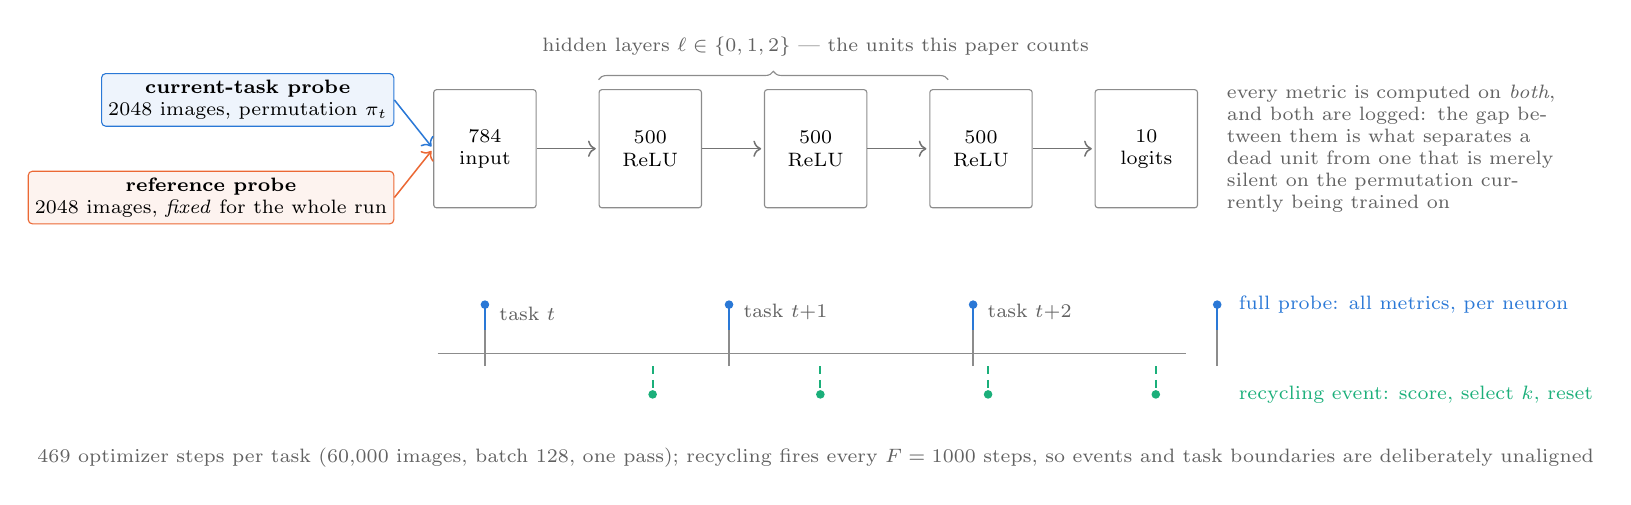
\begin{tikzpicture}[
  font=\small,
  layer/.style = {draw=black!45, rounded corners=1pt, minimum width=13mm,
                  minimum height=15mm, align=center, font=\scriptsize, fill=white},
  probe/.style = {draw=#1, rounded corners=1.5pt, fill=#1!8, align=center,
                  font=\scriptsize, inner sep=2.4pt},
  sub/.style   = {font=\scriptsize, text=black!62},
  ar/.style    = {->, black!55, line width=0.55pt, shorten >=1pt},
]
\definecolor{cCur}{HTML}{2A78D6}
\definecolor{cRef}{HTML}{EB6834}
\definecolor{cEv}{HTML}{1BAF7A}

% ---- the network -------------------------------------------------------------
\node[layer] (in)  at (0,0)   {$784$\\input};
\node[layer] (h1)  at (2.1,0) {$500$\\ReLU};
\node[layer] (h2)  at (4.2,0) {$500$\\ReLU};
\node[layer] (h3)  at (6.3,0) {$500$\\ReLU};
\node[layer] (out) at (8.4,0) {$10$\\logits};
\foreach \a/\b in {in/h1, h1/h2, h2/h3, h3/out} \draw[ar] (\a) -- (\b);

\node[sub, anchor=south] at (4.2,1.05)
  {hidden layers $\ell \in \{0,1,2\}$ --- the units this paper counts};
\draw[decorate, decoration={brace, amplitude=3pt}, black!45]
  (h1.north west) ++(0,0.12) -- ++(4.44,0);

% ---- the two probe batches ---------------------------------------------------
\node[probe=cCur, anchor=east] (pc) at (-1.15,0.62)
  {\textbf{current-task probe}\\$2048$ images, permutation $\pi_t$};
\node[probe=cRef, anchor=east] (pr) at (-1.15,-0.62)
  {\textbf{reference probe}\\$2048$ images, \emph{fixed} for the whole run};
\draw[ar, cCur] (pc.east) -- (in.west);
\draw[ar, cRef] (pr.east) -- (in.west);
\node[sub, anchor=west, text width=42mm] at (9.3,0)
  {every metric is computed on \emph{both}, and both are logged: the gap between
   them is what separates a dead unit from one that is merely silent on the
   permutation currently being trained on};

% ---- the training timeline ---------------------------------------------------
\def\ty{-2.6}
\draw[black!45, line width=0.6pt] (-0.6,\ty) -- (8.9,\ty);
\foreach \x/\lab in {0/{task $t$}, 3.1/{task $t{+}1$}, 6.2/{task $t{+}2$}}{
  \draw[black!45, line width=0.9pt] (\x,\ty-0.16) -- (\x,\ty+0.30);
  \node[sub, anchor=south west] at (\x+0.06,\ty+0.30) {\lab};
}
\draw[black!45, line width=0.9pt] (9.3,\ty-0.16) -- (9.3,\ty+0.30);
\node[sub, anchor=north] at (4.2,\ty-1.08)
  {$469$ optimizer steps per task ($60{,}000$ images, batch $128$, one pass);
   recycling fires every $F=1000$ steps, so events and task boundaries are
   deliberately unaligned};

% probe read-outs at boundaries
\foreach \x in {0, 3.1, 6.2, 9.3}{
  \draw[cCur, line width=0.7pt] (\x,\ty+0.30) -- (\x,\ty+0.62);
  \node[circle, fill=cCur, inner sep=1.1pt] at (\x,\ty+0.62) {};
}
\node[sub, anchor=west, text=cCur] at (9.45,\ty+0.62) {full probe: all metrics, per neuron};

% recycling events
\foreach \x in {2.13, 4.26, 6.39, 8.52}{
  \draw[cEv, line width=0.7pt, densely dashed] (\x,\ty-0.16) -- (\x,\ty-0.52);
  \node[circle, fill=cEv, inner sep=1.1pt] at (\x,\ty-0.52) {};
}
\node[sub, anchor=west, text=cEv] at (9.45,\ty-0.52) {recycling event: score, select $k$, reset};

\end{tikzpicture}
\caption{\textbf{Setting and instrument.} A $784$--$500$--$500$--$500$--$10$
ReLU MLP on online permuted MNIST: each task is a fresh input permutation seen
for a single pass, and the outcome measure is online accuracy, scored on the
forward pass taken \emph{before} each update. Every death metric is evaluated on
two probe batches --- the current task's distribution and a reference
distribution fixed for the entire run --- and per-neuron state is written at
every task boundary. Recycling events are governed by an optimizer-step counter
($F=1000$) rather than by task index, so they fall inside tasks rather than at
their edges.}
\label{fig:arch}
\end{figure}


\paragraph{Calibration, and an honest methods anecdote.}
Our first configurations showed too little plasticity loss to study: at
$\text{lr}=0.01$ the drop from the early to the late window was $1.33\pp$
against the $3\pp$ the pre-registered reproduction gate demanded. The reason is
arithmetic rather than mysterious. \citeauthor{dohare2024loss}'s online permuted
MNIST is genuinely online --- batch size $1$, one example at a time --- so their
setup performs $800 \times 60{,}000 \approx 48$M updates where ours performs
$200 \times (60{,}000/128) \approx 94$k, a factor of $512$ fewer. Plasticity loss
accumulates per update, not per task boundary.

\emph{The correct fix is batch size, and we did not take it}: batch size $1$ at
$200$ tasks does not fit the $11$-hour job ceiling of the compute we had. We
instead followed the pre-registered failure response, which specifies raising
the learning rate first, and climbed a ladder of five values. The drop is
perfectly monotonic in step size across two decades ($-1.18\pp$ at
$\text{lr}=0.001$ to $+4.54\pp$ at $\text{lr}=0.1$; Table~\ref{tab:gate}), which
is \citeauthor{dohare2024loss}'s own finding --- largest step size, strongest
effect --- recovered as a dose--response rather than at a single point. That
monotonicity is what licenses the move: the phenomenon was \emph{present and
under-driven}, not absent, so escalating step size revealed it rather than
manufacturing it. All Setting~1 experiments use $\text{lr}=0.1$. We record the
substitution rather than presenting the learning rate as the natural knob,
because the effective step size that results is high and a reader should be able
to discount for it (Section~\ref{sec:limitations}).

\paragraph{Two further settings.}
\emph{Activation sweep:} ReLU, LeakyReLU, GELU, SiLU and $\tanh$ on the same
task stream, one configuration field. \emph{Convolutional channels:} a small CNN
on label-shuffled CIFAR-10, where the unit is a channel and every metric must
reduce over $(N, H, W)$ rather than $N$. The CIFAR arm's learning-rate
calibration failed --- see Section~\ref{sec:limitations} --- so only its
definitional measurement is reported.

\subsection{The three recycling arms}

% The three recycling arms, side by side. PAPER_BRIEF §8.1: "the single most
% important explanatory diagram in the paper" -- a reader who follows this
% follows the whole experimental logic.
%
% What it has to make unmissable: k is not a design constant. It is read off the
% tau-dormant set at each event, in each layer, and then all three arms recycle
% exactly that many units. What differs across arms is only *which* k.
%
% Geometry note: TMLR's \textwidth is 6.5in = 16.5cm. Everything below is laid
% out to sit inside that -- 12 units at 0.5cm, arm labels to the left, wrapped
% notes to the right -- because a tikzpicture that overflows the margin is a
% silent error that only shows up in the PDF.
\begin{figure}[t]
\centering
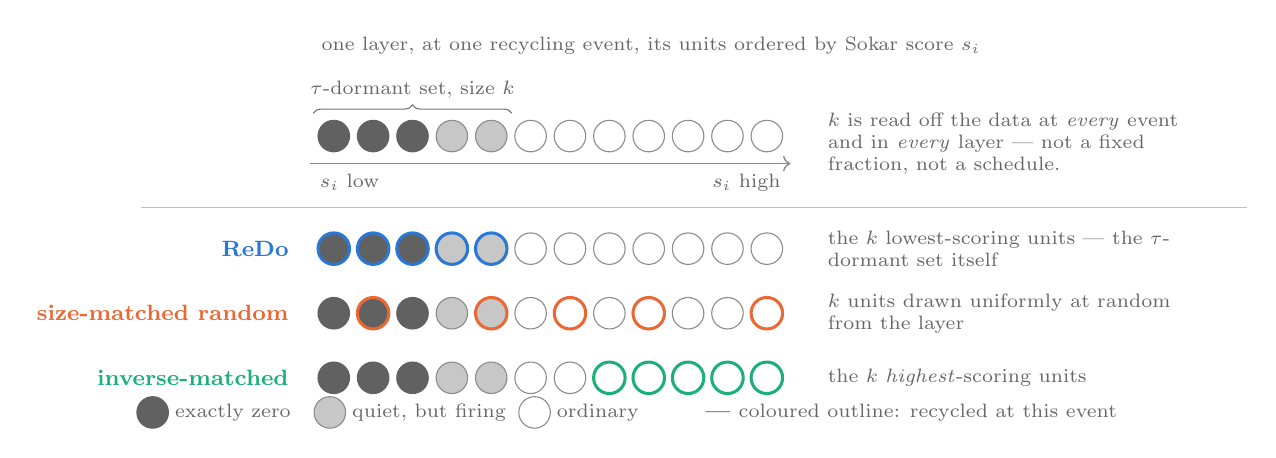
\begin{tikzpicture}[
  font=\small,
  unit/.style   = {circle, draw=black!45, minimum size=4.0mm, inner sep=0pt, line width=0.4pt},
  dead/.style   = {unit, fill=black!62, draw=black!62},
  quiet/.style  = {unit, fill=black!22, draw=black!45},
  alive/.style  = {unit, fill=white},
  pick/.style   = {draw=#1, line width=1.1pt},
  lbl/.style    = {font=\footnotesize\bfseries},
  sub/.style    = {font=\scriptsize, text=black!60},
  note/.style   = {font=\scriptsize, text=black!60, text width=45mm, align=left},
]

\definecolor{cRedo}{HTML}{2A78D6}
\definecolor{cRand}{HTML}{EB6834}
\definecolor{cInv}{HTML}{1BAF7A}

\def\ux{0.50}          % unit pitch
\def\xend{5.50}        % 11 * \ux
\def\xnote{6.15}       % where the right-hand notes start

% ---- the score ordering, shared by all three panels ---------------------------
\node[sub, anchor=west] at (-0.28,2.30)
  {one layer, at one recycling event, its units ordered by Sokar score $s_i$};

\draw[decorate, decoration={brace, amplitude=3pt}, black!55]
  (-0.26,1.44) -- (4*\ux+0.26,1.44)
  node[midway, above, sub, yshift=0.6mm] {$\tau$-dormant set, size $k$};

\foreach \i in {0,...,11}{
  \pgfmathsetmacro\xx{\i*\ux}
  \ifnum\i<3 \node[dead]  at (\xx,1.15) {}; \else
  \ifnum\i<5 \node[quiet] at (\xx,1.15) {}; \else
             \node[alive] at (\xx,1.15) {}; \fi\fi
}
\draw[->, black!45, line width=0.5pt] (-0.30,0.80) -- (\xend+0.30,0.80);
\node[sub, anchor=west] at (-0.30,0.56) {$s_i$ low};
\node[sub, anchor=east] at (\xend+0.30,0.56) {$s_i$ high};

\node[note, anchor=west] at (\xnote,1.05)
  {$k$ is read off the data at \emph{every} event and in \emph{every} layer ---
   not a fixed fraction, not a schedule.};

\draw[black!25, line width=0.4pt] (-2.45,0.24) -- (11.6,0.24);

% ---- the three arms ----------------------------------------------------------
\def\rowy{-0.28}
\foreach \arm/\name/\col/\sel/\note in {%
  0/ReDo/cRedo/{0,1,2,3,4}/{the $k$ lowest-scoring units --- the $\tau$-dormant set itself},
  1/size-matched random/cRand/{1,4,6,8,11}/{$k$ units drawn uniformly at random from the layer},
  2/inverse-matched/cInv/{7,8,9,10,11}/{the $k$ \emph{highest}-scoring units}%
}{
  \pgfmathsetmacro\yy{\rowy - \arm*0.82}
  \node[lbl, anchor=east, text=\col] at (-0.45,\yy) {\name};
  \foreach \i in {0,...,11}{
    \pgfmathsetmacro\xx{\i*\ux}
    \ifnum\i<3 \node[dead]  at (\xx,\yy) {}; \else
    \ifnum\i<5 \node[quiet] at (\xx,\yy) {}; \else
               \node[alive] at (\xx,\yy) {}; \fi\fi
  }
  \foreach \s in \sel {\node[unit, pick=\col] at (\s*\ux,\yy) {};}
  \node[note, anchor=west] at (\xnote,\yy) {\note};
}

% ---- legend ------------------------------------------------------------------
\def\ly{-2.36}
\node[dead]  at (-2.30,\ly) {}; \node[sub, anchor=west] at (-2.14,\ly) {exactly zero};
\node[quiet] at (-0.05,\ly) {}; \node[sub, anchor=west] at ( 0.11,\ly) {quiet, but firing};
\node[alive] at ( 2.55,\ly) {}; \node[sub, anchor=west] at ( 2.71,\ly) {ordinary};
\node[sub, anchor=west] at (4.55,\ly)
  {\,\textbf{---} coloured outline: recycled at this event};

\end{tikzpicture}
\caption{\textbf{The three recycling arms.} At every event, in every layer, the
$\tau$-dormancy score is computed and $k$ is set to the size of the
$\tau$-dormant set. All three arms then recycle exactly $k$ units by the
identical procedure --- re-initialise the incoming weights from the layer's
original initialisation distribution, zero the outgoing weights
\citep{sokar2023dormant} --- and differ only in \emph{which} $k$. Because $k$ is
recomputed per layer per event rather than fixed as a fraction or a schedule,
the comparison isolates the effect of targeting from the effect of dose. Circles
are units; their shading is the state measured on the probe batch, which is
independent of the score that selects them.}
\label{fig:arms}
\end{figure}


ReDo is implemented exactly as specified in \citet{sokar2023dormant}'s
Algorithm~1: every $F = 1000$ optimizer steps, compute $s^\ell_i$ on a
$64$-example batch (their default), then for every unit with $s^\ell_i \le \tau$
re-initialise the incoming weights by sampling from that layer's \emph{original}
initialisation distribution and set the outgoing weights to \emph{zero}. Zeroing
the outgoing weights is what preserves the function the network currently
computes while restoring gradient flow; omitting it turns ReDo into a far more
destructive intervention that still produces plausible-looking curves. A unit
test asserts that at $\tau=0$ the network's outputs are unchanged to numerical
tolerance across a recycling event.

The two controls, and the reason for their design, are the experimental core of
this paper (Figure~\ref{fig:arms}):

\begin{description}
\item[Size-matched random$(\tau)$.] At every event, in every layer, compute the
$\tau$-dormant set, set $k$ to its cardinality, and then recycle $k$ units drawn
\emph{uniformly at random} from that layer by the identical procedure. \emph{$k$
is recomputed at every event and in every layer.} It is not a fixed fraction and
not a schedule.

\item[Inverse-matched$(\tau)$.] The same $k$, but the $k$ \emph{highest}-scoring
units --- the ones least likely to be dead.
\end{description}

The distinction from \citeauthor{sokar2023dormant}'s own random baseline, which
resets a fixed percentage of units on a cosine schedule, is the entire point. A
fixed-percentage baseline varies \emph{how many} units are recycled at the same
time as \emph{which} ones, so a gap between ReDo and that baseline is
attributable to either. Matching cardinality per layer per event removes the
first source of variation, leaving only the second. As it turns out
(Section~\ref{sec:c1}) the realised dose still differs between arms, but in the
direction that works \emph{against} the convenient conclusion, which we report
in full.

\subsection{Pre-registration, statistics, and what was frozen}

\paragraph{What was frozen, and when.} The analysis plan --- outcome measure,
task windows, decision thresholds, seed counts, and the reproduction-gate
criterion --- was committed as \texttt{configs/analysis\_plan.json} at
2026-08-05T14:09:03Z, before any experimental data existed, and was never
edited. The early window is tasks $1$--$10$; the late window is tasks
$151$--$200$; all headline numbers are late-window.

\paragraph{Decision thresholds.} Two, both pre-registered. A difference is
called \emph{no difference} ($\approx$) when its $95\%$ CI contains zero
\emph{and} $|\Delta| < 1\pp$; it is called \emph{much greater} ($\gg$) when
$\Delta > 2\pp$ \emph{and} the CI excludes zero. Anything else is
\emph{inconclusive}, and the pre-specified response to inconclusive is to add
seeds, never to adjust a threshold. We report the rule's verdict and the effect
size together throughout, including where the rule's verdict is unhelpful
(Section~\ref{sec:c1}).

\paragraph{Statistics.} The interquartile mean with stratified bootstrap $95\%$
confidence intervals, $10{,}000$ replicates, resampling seeds independently
within each task column \citep{agarwal2021deep}. Never a bare mean over seeds.
Arm comparisons are \emph{paired}: seed $s$ of every arm starts from the
identical initialisation and sees the identical task stream, so the bootstrap
resamples the same seed indices from both arms, which removes the
initialisation variance that would otherwise swamp a one-point effect.

\paragraph{Calibration is separated from pre-registration.} Learning rate, batch
size, width, depth, number of tasks and dataset are \emph{calibrated}, and every
change to them is recorded with a date and a reason in a deviations log before
the run. Calibrating a setting so that the phenomenon under study is present at
all is a manipulation check; the published work being replicated calibrated its
own setting the same way. What must not move, and did not, are the outcome
measure and the thresholds by which it is judged.

\paragraph{Determinism.} Seeded \texttt{torch}, \texttt{numpy} and \texttt{random};
\texttt{cudnn.deterministic}; weight resampling performed on CPU so that a
recycling event is identical across hardware. This is demonstrated rather than
asserted: on three separate occasions a set of configurations was accidentally
re-executed in a fresh session, twice on different hardware and once on a
different account, and every run reproduced \emph{bit-identically} --- every
online-accuracy value equal at \texttt{atol=0}.

%==============================================================================
\section{Results}
\label{sec:results}
%==============================================================================

\subsection{C1: ReDo's benefit does not require targeting dead units}
\label{sec:c1}

\begin{figure}[t]
\centering

\includegraphics[width=0.68\linewidth]{figures/fig1_tau_sweep.pdf}
\caption{\textbf{The dormancy threshold changes what gets recycled far more than
it changes the result.} \emph{Upper:} late-window online accuracy against $\tau$
for the three arms, with the no-intervention baseline as a reference band.
\emph{Lower:} the pre-registered headline quantity --- of the units actually
recycled, the fraction that were exactly zero on the probe batch, pooled over
layers and events. Over the full $\tau$ range ReDo's target set goes from
$31.4\%$ dead to $12.3\%$ dead, a factor of $2.5$, while its accuracy moves
$0.169\pp$ \ci{0.143}{0.196} --- real, but $3.6\%$ of the $+4.76\pp$ that
recycling buys over doing nothing. Each point is $10$ seeds; bands are
stratified bootstrap $95\%$ CIs. Composition is shown on the current-task probe
batch, as the frozen plan specifies; on the fixed reference batch the same
quantity runs $27.6\% \to 13.5\%$.}
\label{fig:tau}
\end{figure}

\begin{table}[t]
\centering
\caption{The $\tau$-sweep: $190$ runs, $4$ arms, $6$ thresholds, $10$ seeds,
$\text{lr}=0.1$. Late-window online accuracy; the no-intervention baseline is
$87.683\%$ \ci{87.634}{87.730}. ``dead share'' is the pre-registered headline
quantity, the exactly-zero fraction of the set actually recycled. ``$k$'' is the
mean number of units recycled per layer per event --- the realised dose.
Differences are paired IQM with stratified bootstrap $95\%$ CIs. Every
\emph{vs.\ none} entry clears the pre-registered $\gg$ bar.}
\label{tab:tau}
\small
\begin{tabular}{@{}l r r r r r r@{}}
\toprule
& \multicolumn{3}{c}{\textbf{ReDo}} & \multicolumn{3}{c}{\textbf{Size-matched random}} \\
\cmidrule(lr){2-4}\cmidrule(lr){5-7}
$\tau$ & acc.\ (\%) & $\Delta$ vs.\ none & dead share & acc.\ (\%) & $\Delta$ vs.\ none & dead share \\
\midrule
$0$      & 92.438 & $+4.755$ & $31.4\%$ & 92.058 & $+4.375$ & $13.4\%$ \\
$0.01$   & 92.482 & $+4.799$ & $26.5\%$ & 92.062 & $+4.379$ & $12.6\%$ \\
$0.025$  & 92.516 & $+4.832$ & $22.8\%$ & 92.071 & $+4.387$ & $11.9\%$ \\
$0.05$   & 92.535 & $+4.852$ & $19.7\%$ & 92.072 & $+4.389$ & $11.4\%$ \\
$0.1$    & 92.555 & $+4.872$ & $16.6\%$ & 92.053 & $+4.370$ & $10.5\%$ \\
$0.25$   & 92.607 & $+4.924$ & $12.3\%$ & 92.001 & $+4.318$ & $9.2\%$ \\
\midrule
& \multicolumn{3}{c}{\textbf{Inverse-matched}} & \multicolumn{3}{c}{\textbf{ReDo $-$ random, paired}} \\
\cmidrule(lr){2-4}\cmidrule(lr){5-7}
$\tau$ & acc.\ (\%) & $\Delta$ vs.\ none & dead share & $\Delta$ (pp) & $95\%$ CI & frozen verdict \\
\midrule
$0$      & 90.694 & $+3.011$ & $3.9\%$ & $+0.380$ & \ci{0.346}{0.415} & inconclusive \\
$0.01$   & 90.728 & $+3.045$ & $3.7\%$ & $+0.419$ & \ci{0.384}{0.454} & inconclusive \\
$0.025$  & 90.790 & $+3.106$ & $4.1\%$ & $+0.445$ & \ci{0.405}{0.483} & inconclusive \\
$0.05$   & 90.817 & $+3.134$ & $4.2\%$ & $+0.463$ & \ci{0.426}{0.501} & inconclusive \\
$0.1$    & 90.871 & $+3.188$ & $4.3\%$ & $+0.502$ & \ci{0.463}{0.540} & inconclusive \\
$0.25$   & 90.992 & $+3.309$ & $4.4\%$ & $+0.606$ & \ci{0.568}{0.647} & inconclusive \\
\bottomrule
\end{tabular}
\end{table}

\paragraph{Recycling works, which is worth establishing first.}
Whether ReDo helps at all in continual supervised learning had not been tested.
It does: $+4.76$ to $+4.92\pp$ over the no-intervention baseline at every $\tau$,
every CI excluding zero, all far past the pre-registered $\gg$ threshold
(Table~\ref{tab:tau}). It also strongly suppresses dead units --- $\dexact$
falls from $20.8\%$ to $1.5$--$2.2\%$ and effective rank rises from $100$ to
$165$--$192$. Stated on their own, those two numbers are exactly consistent with
``ReDo works by preventing death'', and we state them plainly rather than
burying them, because the rest of this section is the argument that they are
not the mechanism.

\paragraph{The pre-registered C1 pattern fires.}
The plan specified in advance that if accuracy improves with $\tau$ while the
truly-dead fraction of the recycled set falls, C1 is confirmed. That is what
happens: dead share $31.4\% \to 12.3\%$, accuracy $92.438 \to 92.607$. But the
honest reading is stronger than the pattern and weaker than the slope. Across
the entire $\tau$ range ReDo gains $+0.169\pp$ \ci{0.143}{0.196} --- $3.6\%$ of
the $+4.76\pp$ it gains by being switched on at all. Widen the threshold by a
factor of $25$, halve the fraction of the target set that is genuinely dead, and
almost nothing happens to the result.

\paragraph{The control: random selection recovers $88$--$92\%$ of the benefit.}
Size-matched random recycling gains $+4.32$ to $+4.39\pp$ over baseline against
ReDo's $+4.76$ to $+4.92\pp$. It recovers $92.0\%$ of ReDo's benefit at $\tau=0$
and $87.7\%$ at $\tau=0.25$, while the sets it recycles are $86.6$--$90.8\%$
alive and its mean selected Sokar score is $1.00$ at every $\tau$ --- exactly the
layer average, which is what uniform selection must produce and which we use as
an instrument check.

\emph{We do not claim this gap is zero.} ReDo beats size-matched random by
$0.380$ to $0.606\pp$ with every CI excluding zero. Targeting contributes
something real. It contributes roughly a tenth of the total effect; the other
nine tenths are obtained by recycling units chosen at random, nine in ten of
which were alive.

\paragraph{The frozen rule returns \emph{inconclusive}, and we report that.}
Neither pre-registered branch fires for ReDo versus random: $|\Delta|$ is far
below the $2\pp$ bar for $\gg$, but every CI excludes zero so it does not
qualify as $\approx$ either. We record, without acting on it, that the
pre-specified response --- add seeds --- cannot change this verdict: the CIs are
already $\pm 0.04\pp$ and more seeds tighten them, while $\approx$ requires a CI
containing zero, which no amount of power produces for a true nonzero effect.
That is a limitation of the decision rule, not a result, and we report the
rule's verdict beside the effect size rather than amending a plan that was
frozen for exactly this reason.

\paragraph{Inverse-matched: the pre-registered sanity check failed, and the
failure is the strongest evidence in the section.}
The plan predicted that recycling the $k$ \emph{highest}-scoring units would
collapse performance, replicating \citeauthor{sokar2023dormant}'s Figure~15. It
does not collapse. Recycling the units least likely to be dead --- mean selected
score $\approx 2.0$, only $3.9\%$ of them exactly zero --- still beats the
baseline by $+3.01$ to $+3.31\pp$, every CI excluding zero, recovering
$63$--$67\%$ of ReDo's benefit. The arm designed to be maximally destructive
captures two thirds of the effect. We report this as a domain difference from
their RL setting rather than as a bug: the composition table confirms the arm
recycled the units it was meant to, and the same code path produced the other
two arms.

Ordering the three arms by how dead their target sets are gives a monotone
relationship with benefit --- ReDo ($12$--$31\%$ dead, $+4.8\pp$), random
($9$--$13\%$, $+4.4\pp$), inverse ($\approx 4\%$, $+3.2\pp$). So targeting is not
nothing. But the whole span from ``almost entirely alive'' to ``as dead as the
method can find'' is worth $1.7\pp$ against a $4.8\pp$ effect.

\paragraph{The dose confound runs the wrong way, twice.}
The obvious alternative explanation is that ReDo simply perturbs more. It does
not. Because $k$ is recomputed from each run's own state, and because the arms'
networks diverge, the realised dose differs: size-matched random recycles
$131$ units per layer per event at $\tau=0$ against ReDo's $101$ ($+30\%$), and
inverse-matched recycles $247$ ($2.4\times$). Both controls received a
\emph{larger} perturbation and did \emph{worse}. Whatever ReDo's small advantage
is, it is not dose.

This is a design consequence worth naming: matching $k$ within a run to that
run's own dormant set is what the pre-registration specified, and once the arms
diverge their dormant counts diverge too. A \emph{yoked} control --- replaying
ReDo's per-event $k$ into the random arm --- would remove even this, and is the
cleaner design for future work. It would tighten the comparison in the direction
that already favours our conclusion.

\paragraph{Robustness.} The composition is stable across training rather than an
early-training artefact: at $\tau=0$ the dead share of ReDo's recycled set is
$28.3\%$ over tasks $1$--$25$ and $32.3\%$ over tasks $126$--$200$. And even at
$\tau=0$ --- \citeauthor{sokar2023dormant}'s ``only provably dead units''
setting --- ReDo recycles $20.1\%$ of the entire network, of which $68.6\%$ is
alive. That gap is not ours: it arises because the selection score is computed
on their default $64$-example batch while $\dexact$ is measured on $2048$. The
$64$-example default is doing a great deal of unexamined work.

\subsection{C2: the definitions do not measure one thing}
\label{sec:c2}

\begin{figure}[t]
\centering

\includegraphics[width=0.9\linewidth]{figures/fig2_c2_definitions.pdf}
\caption{\textbf{Three published definitions, one set of activations, per
layer.} All quantities are computed on the same forward pass over the same
$2048$-example probe batch, so the spread between them is definitional, not
statistical.}
\label{fig:c2}
\end{figure}

\paragraph{A factor of $3.5$ on identical activations.}
At the operative setting ($\text{lr}=0.1$, late window, no intervention), the
same activations yield: $\dexact$ $20.7\%$; $\dabs$ at $a=10^{-6}$ $20.7\%$, at
$10^{-4}$ $25.7\%$, at $10^{-2}$ $64.7\%$; $\ddorm$ at $\tau=0.1$ ---
ReDo's operating point --- $64.9\%$, at $\tau=0.25$ $72.6\%$. A reader told
``$21\%$ of this network is dead'' and a reader told ``$65\%$ of this network is
dormant'' are being told about the same network in the same state.

\paragraph{It is not an artefact of a collapsed layer.}
A wholly dead layer would make $s^\ell_i$ degenerate ($0/0$, defined as $0$),
flagging every unit in it as dormant at every $\tau$ and inflating the pooled
figure. That is not what is happening. The per-layer $\ddorm[0.1]$ breakdown is
$75.3\% / 54.9\% / 64.2\%$ across the three hidden layers, with $\dexact$ at
$27.9\% / 12.8\% / 20.9\%$; no layer is close to wholly dead
(Figure~\ref{fig:c2}).

\begin{table}[t]
\centering
\caption{\textbf{Change the activation function and the definitions stop
agreeing.} Late window, $25 + 15$ runs. The $\tanh$ row is at its own calibrated
learning rate; at $\text{lr}=0.1$ $\tanh$ diverges to chance and is excluded
from every table and figure. ``---'' marks $\dsat$ as undefined for unbounded
activations, which is what the code returns; reporting $0$ there would be a
category error. Drop is early minus late window.}
\label{tab:acts}
\small
\begin{tabular}{@{}l r r r r r r r@{}}
\toprule
activation & lr & late acc.\ (\%) & drop (pp) & $\dexact$ & $\ddorm[0.1]$ & $\dabs[10^{-2}]$ & $\dsat$ \\
\midrule
ReLU        & $0.1$  & $87.71$ & $4.51$ & $20.67\%$ & $64.90\%$ & $64.71\%$ & --- \\
LeakyReLU   & $0.1$  & $90.05$ & $2.31$ & $\mathbf{0.00\%}$ & $4.62\%$ & $0.00\%$ & --- \\
GELU        & $0.1$  & $88.44$ & $\mathbf{4.82}$ & $\mathbf{0.00\%}$ & $19.08\%$ & $20.49\%$ & --- \\
SiLU        & $0.1$  & $89.70$ & $3.22$ & $\mathbf{0.00\%}$ & $1.14\%$ & $1.54\%$ & --- \\
\midrule
$\tanh$     & $0.003$ & $87.65$ & $0.48$ & $0.00\%$ & $0.00\%$ & $0.00\%$ & $0.00\%$ \\
$\tanh$     & $0.01$  & $88.42$ & $2.71$ & $0.00\%$ & $0.00\%$ & $0.00\%$ & $1.24\%$ \\
$\tanh$     & $\mathbf{0.03}$ & $\mathbf{79.11}$ & $\mathbf{13.00}$ &
$\mathbf{0.00\%}$ & $\mathbf{0.00\%}$ & $\mathbf{0.00\%}$ & $\mathbf{13.84\%}$ \\
\bottomrule
\end{tabular}
\end{table}

\paragraph{The $\tanh$ result.}
At its calibrated learning rate ($0.03$, chosen by the same dose--response ladder
used for the main setting), a $\tanh$ network loses $13.00\pp$ of online accuracy
from the early to the late window --- the largest plasticity loss of any
configuration in this study, larger than any ReLU arm --- while ending at
$79.11\%$, nowhere near the $10\%$ chance level that would indicate mere
divergence. And $\dexact$, $\ddorm$ at every $\tau$, and $\dabs$ at every $a$
all report \textbf{exactly $0.00\%$}. Only $\dsat$ sees anything at all
($13.84\%$ on the current-task probe, $25.87\%$ on the reference probe), and
$\dsat$ is undefined for every activation function used by the four papers this
work engages.

A network can therefore lose more plasticity than any ReLU configuration we
measure and contain, by all three of the field's published definitions, not one
dead unit. This is the single strongest demonstration in the paper that the
metrics are not tracking one underlying quantity. It also means the reproduction
gate's dead-unit criterion is unsatisfiable for $\tanh$ at any learning rate ---
$\dexact$ is identically zero, so its rank correlation with task index is zero by
construction --- which is the dissociation case the pre-registered plan says to
stop and report rather than work around.

\paragraph{Smooth activations: weaker than ``by construction'', and
dtype-dependent.}
Under GELU and SiLU, $\dexact$ is $0.00\%$ while $\ddorm[0.1]$ flags $19.1\%$ and
$1.1\%$ respectively and $\dabs[10^{-2}]$ flags $20.5\%$ and $1.5\%$. GELU has
the \emph{largest} plasticity drop of the four unbounded activations
($4.82\pp$) and, by the \emph{Nature} paper's definition, no dead units at all.

The mechanism deserves care, because the intuitive claim is wrong in an
instructive way. For SiLU the vanishing of $\dexact$ genuinely is by
construction: $\sigma(x)$ requires $x \approx -90$ before it underflows, which
nothing reaches. For GELU it is not. $\mathrm{GELU}(x) = x\Phi(x)$, and in
float32 $1 + \mathrm{erf}(x/\sqrt{2})$ rounds to zero at $x \le -5.55$, a
pre-activation trained networks reach routinely --- so GELU units \emph{can}
register as exactly dead, through a floating-point underflow. The threshold is
$-5.55$ in float32 and $-8.40$ in float64: the same unit, same weights, same
inputs, is dead in one precision and alive in the other. Our trained GELU
networks did not reach it, so the measured value is $0.00\%$, but the reason is
empirical rather than definitional. A death metric whose value depends on
floating-point precision is not measuring a property of the network.

\paragraph{Convolutional channels.}
In a convolutional layer the unit is a channel and its activation is a feature
map, so ``dead'' must mean zero across all inputs \emph{and} all spatial
positions. Under that generalisation, in the three convolutional layers of a
small CNN on label-shuffled CIFAR-10, $\dexact$ finds $0.00\%$, $0.91\%$ and
$0.00\%$ of channels dead while $81$--$88\%$ of all spatial positions in those
layers are silent, and $\ddorm[0.1]$ flags $21$--$35\%$. The fully-connected
layer in the same network reports $26.3\%$ dead. The definition is therefore not
merely activation-dependent but layer-type-dependent: a channel can be $88\%$
spatially silent and still count as fully alive. \emph{This measurement is
reported on its own}; the CIFAR arm's learning-rate calibration failed
(Section~\ref{sec:limitations}), so no plasticity or intervention result from
that setting is used anywhere in this paper. A statement about what a definition
counts does not require the network to be losing plasticity.

\paragraph{Death is partly distribution-relative.}
\begin{figure}[t]
\centering
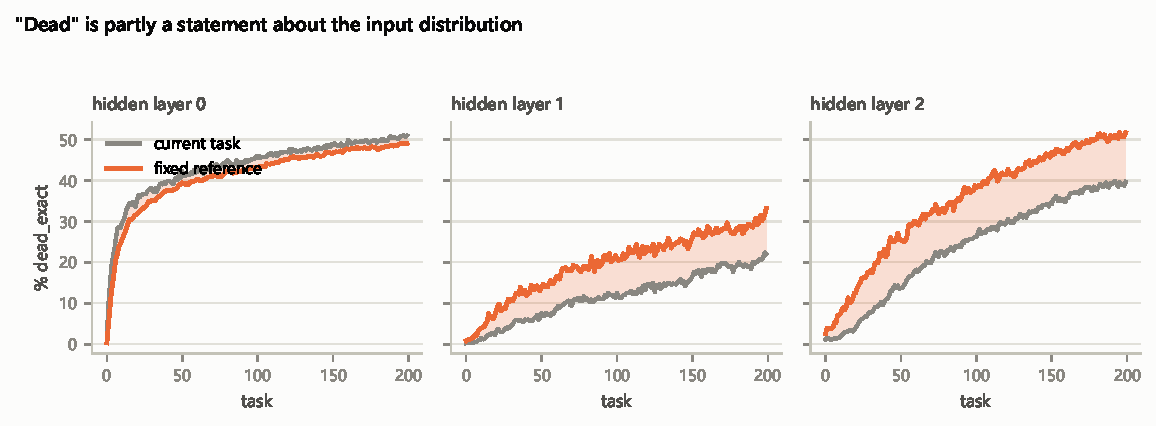
\includegraphics[width=0.9\linewidth]{figures/fig6_reference_asymmetry.pdf}
\caption{\textbf{$\dexact$ measured on the current task's distribution versus a
fixed reference distribution, per layer.} The two agree in layers $0$ and $1$
and diverge sharply in the last hidden layer. Distribution-relative death is a
last-layer phenomenon, which is a sharper claim than the pooled figure.}
\label{fig:refasym}
\end{figure}
Comparing the two probe batches at $\text{lr}=0.1$: pooled $\dexact$ is $20.7\%$
on the current task's distribution and $26.0\%$ on the fixed reference. Units
stay alive for the permutation currently being trained on and fall silent on a
distribution the network has not seen recently. Per layer the effect localises
completely: $27.9\%$ vs.\ $26.9\%$ (layer $0$) and $12.8\%$ vs.\ $12.1\%$ (layer
$1$) show no gap, while layer $2$ reads $20.9\%$ vs.\ $37.2\%$
(Figure~\ref{fig:refasym}). None of the four source papers can observe this,
because none of them probes a second, fixed distribution. Section~\ref{sec:c4}
shows the same asymmetry dominating a much larger quantity.

\subsection{C3: helping plasticity while killing more neurons}
\label{sec:c3}

\begin{table}[t]
\centering
\caption{\textbf{The two anomalies, replicated.} $35$ runs, $5$ seeds,
$\text{lr}=0.1$, late window. $\Delta$ is paired against plain backpropagation.
$\dexact$ is given on both probe batches because the C3 claim should not depend
on that choice, and does not.}
\label{tab:c3}
\small
\begin{tabular}{@{}l r r l r r r@{}}
\toprule
arm & acc.\ (\%) & $\Delta$ (pp) & $95\%$ CI & $\dexact$ cur.\ & $\dexact$ ref.\ & erank \\
\midrule
plain backprop        & $87.71$ & --- & --- & $20.67\%$ & $26.02\%$ & $100.2$ \\
\textbf{$L_2$, $\lambda{=}10^{-4}$} & $\mathbf{89.22}$ & $\mathbf{+1.50}$ & \ci{1.41}{1.59} & $\mathbf{40.17\%}$ & $\mathbf{49.36\%}$ & $\mathbf{50.1}$ \\
$L_2$, $\lambda{=}10^{-3}$ & $85.34$ & $-2.38$ & \ci{-2.65}{-2.11} & $66.52\%$ & $72.47\%$ & $14.5$ \\
$L_2$, $\lambda{=}10^{-2}$ & $75.85$ & $-11.86$ & \ci{-12.70}{-11.04} & $60.38\%$ & $66.20\%$ & $7.1$ \\
shrink \& perturb     & $89.66$ & $+1.94$ & \ci{1.87}{2.02} & $7.18\%$ & $6.76\%$ & $46.3$ \\
dropout $0.1$         & $83.31$ & $-4.40$ & \ci{-4.51}{-4.30} & $22.45\%$ & $31.90\%$ & $109.9$ \\
\textbf{online normalisation} & $\mathbf{90.87}$ & $\mathbf{+3.16}$ & \ci{3.08}{3.23} & $\mathbf{28.61\%}$ & $\mathbf{39.73\%}$ & $146.4$ \\
\bottomrule
\end{tabular}
\end{table}

\begin{figure}[t]
\centering
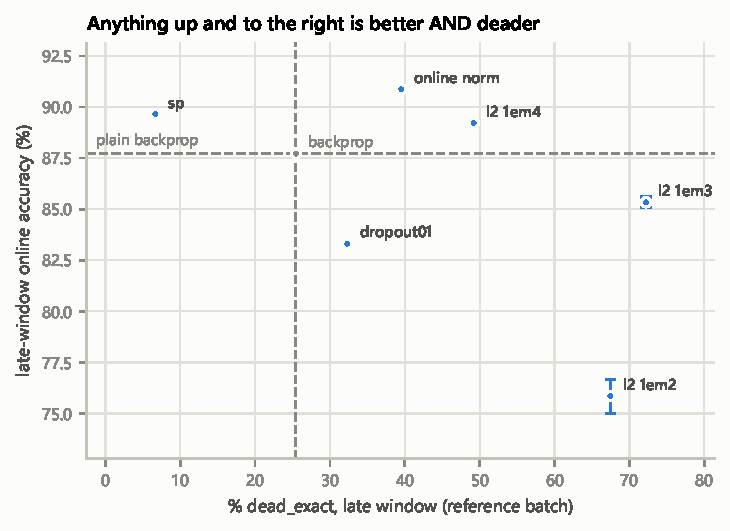
\includegraphics[width=0.62\linewidth]{figures/fig7_c3_anomaly.pdf}
\caption{\textbf{The C3 dissociation is two-dimensional.} Accuracy against dead
units, one point per arm. If dead units were the pathology, the arms would lie
on a downward line. $L_2$ at its beneficial dose and online normalisation are
both up and to the right --- better \emph{and} deader.}
\label{fig:c3}
\end{figure}

Both target observations pre-registered for this experiment fire
(Table~\ref{tab:c3}, Figure~\ref{fig:c3}).

\paragraph{$L_2$ improves accuracy while nearly doubling dead units.}
At $\lambda = 10^{-4}$, $L_2$ regularisation gains $+1.50\pp$ \ci{1.41}{1.59}
over plain backpropagation while $\dexact$ rises from $20.67\%$ to $40.17\%$ and
effective rank falls from $100.2$ to $50.1$. Higher accuracy, nearly twice the
dead units, half the effective rank. The same holds on the reference probe
($26.02\% \to 49.36\%$), so the anomaly is not an artefact of which distribution
is used to probe.

The dose--response sharpens the point rather than softening it. Accuracy is an
inverted U in $\lambda$: $10^{-4}$ helps, $10^{-3}$ costs $2.38\pp$, $10^{-2}$
costs $11.86\pp$. Dead units are \emph{not} monotone either --- they peak at
$\lambda = 10^{-3}$ ($66.5\%$) and fall back at $10^{-2}$ ($60.4\%$), by which
point effective rank has collapsed to $7.1$ and the network is simply small. So
the anomaly is specifically that \emph{within the beneficial dose} the two
quantities move in opposite directions. That is a stronger and more awkward
statement than ``$L_2$ increases death''.

\paragraph{Online normalisation increases the pathology it was designed to
prevent.}
Online Normalization \citep{chiley2019online} is the best-performing arm we
measure, at $+3.16\pp$ \ci{3.08}{3.23} over backpropagation --- clearing the
pre-registered $\gg$ threshold, the only C3 arm to do so --- while carrying
$28.61\%$ dead units against backpropagation's $20.67\%$, a $38\%$ increase
($39.73\%$ vs.\ $26.02\%$, a $53\%$ increase, on the reference probe). It also
has the highest effective rank of any arm ($146.4$). The method works; its
stated mechanism is not why.

\paragraph{The counterexample that keeps this honest.}
Shrink-and-perturb \citep{ash2020warm} gains $+1.94\pp$ \emph{and} reduces
$\dexact$ to $7.18\%$. Not every helpful method increases death. This is
precisely why the claim must be stated as a dissociation --- dead-unit count and
plasticity can move independently, in either relative direction --- rather than
as a law that death is good. Dropout is the fourth quadrant: it hurts accuracy
($-4.40\pp$) while barely changing death ($22.45\%$).

\paragraph{Mechanism.}
The pattern across arms is consistent with dead-unit count tracking
\emph{parameter-norm and scale} effects rather than lost capacity. $L_2$ and
online normalisation both act on activation and weight scale; both shift many
units below the exactly-zero threshold; and both improve trainability by keeping
the effective step size in a useful range. Shrink-and-perturb, which
periodically rescales \emph{and} re-randomises, moves scale without pushing units
against the ReLU hinge, and its death count falls. Under this reading a
$\dexact$ count is partly a readout of where a layer's activation distribution
sits relative to zero, which is a scale property, and only partly a readout of
lost capacity --- which is what Section~\ref{sec:c4} independently supports.

\subsection{C4: death is reversible}
\label{sec:c4}

\begin{figure}[t]
\centering

\includegraphics[width=0.98\linewidth]{figures/fig3_c4_survival.pdf}
\caption{\textbf{Neuron mortality as a survival process.} Per-neuron state
logged at every one of $200$ task boundaries, $25$ runs with no intervention of
any kind. \emph{(a)} time to first death; \emph{(b)} probability that a unit dead
at one boundary is alive at the next, on both probe distributions; \emph{(c)}
how long silence lasts.}
\label{fig:surv}
\end{figure}

We logged the full state of every unit --- mean absolute activation, exact-zero
flag on both probes, incoming and outgoing weight norms, per-neuron gradient
norm --- at every one of the $200$ task boundaries, and treat each unit as a
subject in a survival study. The runs analysed here carry \emph{no intervention},
so nothing below can be an artefact of recycling.

\paragraph{A fifth of dead units come back on their own.}
On the fixed reference distribution, a unit that is $\dexact$ at one task
boundary is alive again at the next with probability $21.71\%$
\ci{21.37}{22.21}, pooled across layers, with no intervention applied.

\begin{center}
\small
\begin{tabular}{@{}l r l@{}}
\toprule
layer & $P(\text{dead} \to \text{alive})$, one task later & $95\%$ CI \\
\midrule
$0$ & $4.36\%$ & \ci{4.22}{4.47} \\
$1$ & $39.68\%$ & \ci{38.27}{42.93} \\
$2$ & $29.82\%$ & \ci{29.51}{31.71} \\
\midrule
pooled & $\mathbf{21.71\%}$ & \ci{21.37}{22.21} \\
\bottomrule
\end{tabular}
\end{center}

\paragraph{Death is a state units churn through, not a fate they arrive at.}
$87.3\%$ of all units die at least once, against a late-window prevalence of
only $26\%$. Of the $68{,}440$ death episodes, the median closed episode lasts
$2$ tasks, $46.2\%$ last exactly one task, and only $3.2\%$ are still open at
task $199$.

\paragraph{The first layer is the exception, and should be reported as one.}
Layer $0$'s recovery rate is $4.4\%$ against $30$--$40\%$ in layers $1$ and $2$;
its median closed episode is $4$ tasks against $1$ and $2$; and $12.6\%$ of its
episodes never end, against $2.0\%$ and $2.5\%$. Permanent death is real, but in
this setting it is a first-layer phenomenon. That is consistent with the
mechanism: layer $0$ sees the raw permuted input, so its pre-activations are not
rescued by upstream parameters changing.

\paragraph{Do not quote the current-task version of this number.}
On the current task's probe batch the same quantity reads $59.91\%$
\ci{59.72}{60.22}. That is not a better estimate of revival; it is mostly the
input distribution moving. The permutation changes at every boundary, so a unit
silent on task $t$'s inputs may fire on task $t{+}1$'s without any parameter
having changed. The reference batch is fixed and cannot produce that artefact,
which is why it carries the claim. The gap between $60\%$ and $22\%$ is itself a
C2 result: most of what naively looks like spontaneous recovery is
distribution shift.

\paragraph{Why this matters for the rest of the paper.}
Every method this paper engages is premised on dead units being lost capacity
that has to be actively restored. If a fifth of them restore themselves within
one task, the premise is weakened before any intervention is applied --- and a
recycling method that appears to ``revive'' units is competing against a process
that revives them anyway.

\paragraph{Recycling selects the living.}
\begin{figure}[t]
\centering

\includegraphics[width=0.9\linewidth]{figures/fig4_c4_recurrence.pdf}
\caption{\textbf{Which units recycling keeps choosing, and what state they were
in.} Per-unit recycle counts against a null that holds $k$ fixed per task and
per layer and redraws only \emph{which} units, so any excess concentration is
targeting rather than dose.}
\label{fig:recur}
\end{figure}
Across every recycling event in the sweep, the fraction of the selected set that
was alive is $86.6$--$90.8\%$ for size-matched random and $95.6$--$96.3\%$ for
inverse-matched. The second number is that arm behaving exactly as designed and
is not evidence on its own; its value is that the two arms sit at opposite ends
of the targeting scale, which calibrates the measure. The concentration analysis
(Figure~\ref{fig:recur}) confirms this: on the random arm, per-unit recycle
counts match a same-dose null to three decimals (enrichment $1.001 / 1.005 /
0.999$ across layers, Gini $0.139$--$0.221$ against a null of $0.138$--$0.222$),
which is what a negative control must produce; on the inverse arm the same units
are chosen repeatedly, roughly $5\times$ more concentrated than dose alone
predicts.

\subsection{C5: Adam-induced death is real; its predicted timing is not}
\label{sec:c5}

\begin{table}[t]
\centering
\caption{\textbf{Optimizers.} $20$ runs, $5$ seeds, late window. SGD runs at its
own calibrated learning rate per the protocol, so the SGD-vs-Adam accuracy
comparison is not like-for-like; the Adam-default-vs-Lyle-tuned contrast, at
identical learning rate, is clean.}
\label{tab:c5}
\small
\begin{tabular}{@{}l r r r r r@{}}
\toprule
arm & lr & acc.\ (\%) & drop (pp) & $\dexact$ & erank \\
\midrule
SGD $+$ momentum & $0.1$ & $87.71$ & $4.51$ & $20.67\%$ & $100.2$ \\
Adam, defaults ($\epsilon{=}10^{-8}$, $\beta_2{=}0.999$) & $10^{-3}$ & $90.28$ & $3.19$ & $\mathbf{59.30\%}$ & $50.5$ \\
Adam, tuned ($\epsilon{=}10^{-3}$, $\beta_2{=}0.9$) & $10^{-3}$ & $90.46$ & $2.25$ & $\mathbf{24.60\%}$ & $120.8$ \\
AdamW & $10^{-3}$ & $91.18$ & $2.26$ & $58.37\%$ & $54.9$ \\
\bottomrule
\end{tabular}
\end{table}

\paragraph{The effect is real and large.} Adam at its default hyperparameters
carries $59.30\%$ dead units against SGD's $20.67\%$, with effective rank halved
($50.5$ vs.\ $100.2$). The two-hyperparameter change recommended by
\citet{lyle2023understanding} --- raising $\epsilon$ to $10^{-3}$ and lowering
$\beta_2$ to $0.9$ --- cuts this to $24.60\%$ at an identical learning rate, a
$2.4\times$ reduction, and restores effective rank to $120.8$. AdamW's decoupled
weight decay \citep{loshchilov2019decoupled} does not rescue it ($58.37\%$).

\paragraph{And it dissociates from plasticity, again.} Adam carries roughly
three times SGD's dead units \emph{and} a smaller plasticity drop ($3.19$ vs.\
$4.51\pp$). This is the fourth independent dissociation in the paper. The
accuracy comparison across optimizers is not like-for-like, since the learning
rates differ by design; the dead-unit comparison is, since it is a property of
the activations either way.

\paragraph{The pre-registered timing hypothesis did not confirm. We report it as
a null.}
The plan predicted a death spike in the first steps after each task switch, when
Adam's first-moment estimate $\hat{m}$ has updated aggressively but the
second-moment estimate $\hat{v}$ has not --- the mechanism of
\citet{lyle2023understanding}. To test it we added intra-task probing at
$25$-step resolution, yielding $228{,}000$ probe rows across the C5 runs. Pooling
over tasks $50$--$199$ by steps-since-switch:

\begin{center}
\small
\begin{tabular}{@{}l r r r r r r@{}}
\toprule
arm & step $0$ & $25$ & $50$ & $100$ & $200$ & $450$ \\
\midrule
SGD & $22.94$ & $\mathbf{25.38}$ & $22.95$ & $21.17$ & $19.82$ & $18.40$ \\
Adam, defaults & $63.18$ & $57.42$ & $56.21$ & $55.98$ & $55.94$ & $55.86$ \\
Adam, tuned & $26.91$ & $23.49$ & $23.02$ & $22.87$ & $22.06$ & $20.54$ \\
AdamW & $63.57$ & $57.12$ & $56.08$ & $55.76$ & $55.58$ & $55.38$ \\
\bottomrule
\end{tabular}
\end{center}

\emph{SGD} shows the predicted spike ($+2.44\pp$ at step $25$). Adam does not:
it declines monotonically from the switch onward, which is the reverse of the
hypothesis. Adam-induced death is real but it \textbf{accumulates across tasks}
($25.5\%$ over tasks $0$--$19$, $64.9\%$ over tasks $180$--$199$) rather than
within them. Within a task, Adam's layers move in opposite directions: layer $0$
\emph{gains} dead units over the course of a task ($24.4 \to 27.6\%$) while
layers $1$ and $2$ recover ($76.3 \to 64.2\%$ and $88.8 \to 75.8\%$).

Two limitations could in principle produce this null, and neither affects the
cross-task accumulation result. The probe grid is $25$ steps, so a spike confined
to the first ten steps would be invisible --- SGD's was caught only because it is
broad; a log-spaced grid would settle it. And the reference probe was disabled
for these runs to halve probe cost, so the step-$0$ reading conflates ``the unit
is dead'' with ``the permutation just changed'', which is exactly what the
reference batch exists to separate. Both should be fixed before this null is
treated as final.

\subsection{Summary}

\begin{table}[t]
\centering
\caption{\textbf{Every claim, its effect size, the pre-registered threshold it
was judged against, and the verdict.} Thresholds are from the frozen analysis
plan and were not adjusted after seeing data. ``Inconclusive'' is the plan's own
label for a difference below the $\gg$ bar whose CI excludes zero; where it
appears we report it together with the effect size, since the rule cannot return
$\approx$ for any true nonzero effect.}
\label{tab:summary}
\small
\begin{tabular}{@{}c p{0.34\linewidth} l l l@{}}
\toprule
& claim & effect & pre-registered rule & verdict \\
\midrule
C1 & ReDo's benefit does not come from reviving dead units &
accuracy $+0.169\pp$ across $\tau$ while dead share $31.4\% \to 12.3\%$;
random-matched recovers $88$--$92\%$ &
``accuracy up, dead share down $\Rightarrow$ C1 confirmed'' &
\textbf{supported}; strong form refuted \\
\addlinespace
C1$'$ & ReDo $\gg$ size-matched random &
$+0.38$ to $+0.61\pp$, CI excludes zero &
$\gg$ needs $>2\pp$; $\approx$ needs CI $\ni 0$ &
\textbf{inconclusive} \\
\addlinespace
C1$''$ & inverse-matched collapses (Sokar Fig.~15) &
$+3.01$ to $+3.31\pp$ \emph{above} baseline &
predicted collapse &
\textbf{refuted} \\
\addlinespace
C2 & the definitions disagree materially &
$3.5\times$ spread; $0.00\%$ vs.\ $13.0\pp$ loss under $\tanh$ &
qualitative target observation &
\textbf{established}, six ways \\
\addlinespace
C3 & $L_2$ helps while increasing death; online norm increases what it prevents &
$+1.50\pp$ with $20.7 \to 40.2\%$; $+3.16\pp$ with $20.7 \to 28.6\%$ &
both target observations stated in advance &
\textbf{confirmed}, both \\
\addlinespace
C4 & mortality has characterisable dynamics &
$21.71\%$ \ci{21.37}{22.21} revival; $87.3\%$ ever dead &
analysis-only, no threshold &
\textbf{death is reversible} \\
\addlinespace
C5 & Adam-induced death is a distinct mechanism &
$59.3\%$ vs.\ $20.7\%$; but no post-switch spike &
predicted within-task spike &
\textbf{half}: real, timing \textbf{null} \\
\bottomrule
\end{tabular}
\end{table}

Table~\ref{tab:summary} collects every claim against the threshold it was judged
by. Four independent dissociations between dead-unit count and plasticity appear
across the study: at $\text{lr}=0.001$ dead units nearly triple while accuracy
\emph{improves}; Adam carries three times SGD's dead units with a \emph{smaller}
plasticity drop; GELU has the largest drop of the unbounded activations and
\emph{zero} dead units by the standard metric; and $L_2$ at its beneficial dose
doubles dead units while improving accuracy. Alongside those, C4 shows dead
units returning on their own.

%==============================================================================
\section{Implications for measurement practice}
\label{sec:practice}
%==============================================================================

Each of the following is a change a paper in this area can adopt immediately,
and each follows from a specific result above rather than from general caution.

\begin{enumerate}
\item \textbf{Report a size-matched random control alongside any recycling-based
intervention} --- $k$ recomputed per layer per event, not a fixed percentage and
not a schedule. This is the only design that separates the effect of \emph{which}
units are recycled from \emph{how many}. A fixed-percentage baseline varies both
at once, and the conflation is what produces an inflated impression of targeting
precision: here, the size-matched control recovers $88$--$92\%$ of the benefit
that the targeted method receives credit for.

\item \textbf{Never report a single ``percent dead'' figure without pairing it
with a non-layer-relative measure.} On identical activations, $\ddorm[0.1]$ read
$64.9\%$ where $\dexact$ read $20.7\%$; the difference is quiet-but-firing units,
and one fixed-absolute or exact-zero number reported alongside makes it visible
at a glance instead of requiring a follow-up study. The two measures answer
different questions and neither is a substitute for the other.

\item \textbf{Report death against a fixed reference distribution, not only the
current task's.} The same units read $20.7\%$ dead on the current task's inputs
and $26.0\%$ on a fixed reference, localised almost entirely in the last hidden
layer ($20.9\%$ vs.\ $37.2\%$); and the spontaneous-revival rate reads $60\%$ on
one probe and $22\%$ on the other. A reference probe is the only way to separate
genuine death from distribution-relative silence, and it costs one extra forward
pass per measurement.

\item \textbf{Report the spontaneous revival rate as a baseline before crediting
any method with ``recovering'' capacity.} At a $21.7\%$ per-task baseline with no
intervention at all, some portion of any reset method's apparent restoration is
units that would have come back regardless. This baseline is cheap: it requires
only that per-neuron state be logged at task boundaries, which is a
write, not a computation.

\item \textbf{When evaluating on anything other than ReLU, do not rely on
exact-zero counts.} Under SiLU the count is zero by construction; under GELU it
is zero in practice and, worse, depends on floating-point precision; under
$\tanh$ it is zero while the network saturates. The $\tanh$ result here is the
sharpest case on record: $13.0\pp$ of plasticity lost with three published
definitions all reading exactly $0.00\%$. Report a saturation criterion for
bounded activations and an absolute-magnitude criterion for smooth ones, and
report exact-zero as \emph{undefined} rather than $0$ where it does not apply.
\end{enumerate}

%==============================================================================
\section{Discussion}
\label{sec:discussion}
%==============================================================================

\paragraph{The thread.} The field measures a proxy that is sometimes present
without the pathology and sometimes absent despite it. Present without it: $L_2$
at its beneficial dose, online normalisation, and Adam all carry more dead units
than the baselines they beat. Absent despite it: GELU has the largest plasticity
drop of the unbounded activations with $\dexact$ at zero, and $\tanh$ loses
$13.0\pp$ with three definitions at zero. A quantity that behaves this way is not
a measurement of lost capacity. It is closer to a readout of where a layer's
activation distribution currently sits relative to the origin --- a scale
property, which is why interventions that act on scale ($L_2$, normalisation,
Adam's per-parameter rescaling) move it so reliably in either direction.

\paragraph{What this does and does not say about recycling methods.} They work.
ReDo gains $+4.8\pp$ in our setting, which had not previously been shown for
continual supervised learning at all, and it does suppress dead units and lift
effective rank substantially. Nothing here argues for abandoning them. What the
evidence does not support is the stated mechanism. Recycling units chosen
uniformly at random, roughly nine in ten of which are alive, recovers nearly all
of the benefit; recycling the units \emph{least} likely to be dead recovers two
thirds. The natural reading is that the operative ingredient is the
perturbation --- re-randomised incoming weights with zeroed outgoing weights,
applied periodically, which resets a subspace of the parameters without changing
the function --- and that the dormancy score is a convenient way to choose where
to apply it rather than the reason it works. That is consistent with
\citet{klein2024plasticity}'s survey finding that generic regularisation
outperforms dormancy-targeted intervention, and with
\citet{lyle2024disentangling}'s decomposition into multiple mechanisms on which
single-target interventions are individually insufficient.

\paragraph{Relation to prior negative results.} Our findings line up with the
three counter-results scattered through the literature rather than contradicting
them. \citeauthor{sokar2023dormant}'s observation that pruning dormant units is
free is what one expects if those units are not carrying recoverable capacity.
\citeauthor{lyle2023understanding}'s plasticity loss without saturated units is
the same dissociation we measure four more times.
\citeauthor{kooi2024hadamard}'s sign reversal under $\tanh$ is the phenomenon our
$\tanh$ arm isolates to the definition itself. Where we diverge is on
inverse-matched recycling, which \citeauthor{sokar2023dormant} report as
collapsing and we find beats baseline by $3\pp$. We treat that as a domain
difference between supervised continual learning and their RL setting rather
than as a correction to their result; the arm ran correctly, and its composition
table confirms it recycled the units it was meant to.

\paragraph{Threats to validity.} The primary setting is one architecture family
on one task stream, and the effective step size ($\text{lr}=0.1$ with momentum
$0.9$) is high. The most important guard against reading too much into that is
that the central claims are dissociations --- pairs of quantities moving in
opposite directions --- rather than absolute levels, and they appear at five
learning rates spanning two decades, four activation functions, four optimizers,
two probe distributions, and both a fully-connected and a convolutional
architecture. A confound that produced all of those in the same direction would
have to be unusually accommodating. The claim most exposed to setting is the
magnitude of ReDo's advantage over random-matched, which is small and could
plausibly be a different small number elsewhere; the claim least exposed is that
the definitions disagree, which is arithmetic on a single forward pass.

%==============================================================================
\section{Limitations}
\label{sec:limitations}
%==============================================================================

\begin{itemize}
\item \textbf{Architecture.} An MLP, plus a small CNN for the channel-level
definitional measurement. No large-scale vision or language model.

\item \textbf{Task streams.} Online permuted MNIST and label-shuffled CIFAR-10.
Both are synthetic non-stationarity of a kind the plasticity literature uses
routinely, but neither is a natural distribution shift.

\item \textbf{No transformer arm, and the reason.} We considered and cancelled
one. For a gated unit --- SwiGLU computes
$(W_1x) \odot \sigma(W_2 x)$ --- ``the neuron is dead'' is not well defined:
gate-death, value-death and product-death are three different events with
different gradient consequences, and no definition covering them exists in the
literature. Inventing one is a separate paper, and using a wrong one here would
undercut the very argument we are making about definitional care. The three
works this paper engages most closely use permuted MNIST, small CNNs and DQN
respectively, so this is not a lower bar than the literature being examined ---
but it is a real open problem and we state it as one.

\item \textbf{Effective step size.} $\text{lr}=0.1$ with momentum $0.9$ is high.
It was reached by the pre-registered failure ladder, and it is a substitute for
the correct fix, which was to reduce batch size toward the fully online regime of
\citet{dohare2024loss} (Section~\ref{sec:setup}). The dose--response is monotone
across two decades of step size, so we do not think the phenomenon is an artefact
of the endpoint, but a reader should discount accordingly.

\item \textbf{The CIFAR arm failed calibration and its plasticity results are
not reported.} At $\text{lr}=0.01$ over $50$ tasks accuracy \emph{rose}
($45.1\% \to 56.6\%$), so there was no plasticity loss for recycling to address;
at $\text{lr} \in \{0.03, 0.1\}$ over $200$ tasks the network collapsed entirely
by task $30$ --- loss exactly $\ln 10$, gradient norm zero in every layer, the
fully-connected layer $99.8$--$100\%$ dead. No usable learning rate was found,
so only the channel-level definitional measurement from that setting is used.
This also exposed a real limitation of our own frozen gate: a totally collapsed
network satisfies ``accuracy fell by $\ge 3\pp$'' and ``dead units rose''
\emph{maximally}, so collapse produces the most emphatic possible pass. We
report this rather than amending the plan, and added a separate advisory health
check (accuracy at chance, loss at $\ln n_{\text{classes}}$, gradient norm zero)
that runs alongside the frozen verdict without changing it.

\item \textbf{The C5 timing hypothesis did not confirm}, with two identified
weaknesses in the test itself (a $25$-step probe grid, and the reference probe
disabled for those runs). Section~\ref{sec:c5}.

\item \textbf{Boundary resolution in the survival analysis.} Per-neuron state is
logged at task boundaries, and recycling fires every $1000$ steps against $469$
steps per task, so a unit that died and revived \emph{within} a task is
invisible. The revival rates in Section~\ref{sec:c4} are therefore lower bounds.

\item \textbf{$\dexact$ is a knife edge.} A unit whose pre-activation sits just
below zero on every reference input crosses back on a small weight change. That
is arguably the finding rather than a flaw --- it is a property of the field's
definition --- but a robustness pass with $\dabs$ at $10^{-4}$ would settle
whether the revived units are predominantly the marginal ones. The logged data
retains \texttt{mean\_abs\_act} at float64 precisely so this can be done without
re-running anything.

\item \textbf{The controls are matched within a run, not yoked across arms.} As
described in Section~\ref{sec:c1}, this leaves a residual dose difference of
$30$--$150\%$ between arms. It runs against our conclusion in every case, so it
is conservative here, but a yoked design is cleaner.
\end{itemize}

%==============================================================================
\section{Conclusion}
%==============================================================================

Four claims, stated as they were in the introduction and now with their
evidence attached.

\textbf{ReDo's benefit does not require targeting dead units.} Across the full
$\tau$ range the genuinely dead share of the recycled set falls from $31.4\%$ to
$12.3\%$ while accuracy moves $0.169\pp$, $3.6\%$ of the benefit of recycling at
all. A control matched in size --- not percentage, size, recomputed per layer at
every event --- recovers $88$--$92\%$ of the benefit while recycling sets that
are $87$--$91\%$ alive, and recycling the highest-scoring units recovers two
thirds. Targeting contributes on the order of a tenth of the effect; the
remainder is unrelated to which units are chosen.

\textbf{The field's death metrics disagree by a factor of $3.5$ on identical
activations,} systematically rather than noisily, with each definition's blind
spot traceable to a specific design choice --- and under $\tanh$ three of the four
report exactly $0.00\%$ on a network that has lost $13.0\pp$ of plasticity.

\textbf{Two anomalies reported inside a \emph{Nature} paper replicate and are
given a mechanism:} $L_2$ at its beneficial dose improves accuracy while nearly
doubling dead units and halving effective rank, and online normalisation is the
best-performing method we measure while carrying $38\%$ more of the units it was
designed to prevent. Both are consistent with dead-unit count acting as a readout
of activation scale rather than of lost capacity.

\textbf{A fifth of dead units revive with no intervention at all} --- $21.71\%$
within one task on a fixed reference distribution, with $87.3\%$ of units dying
at least once against a $26\%$ steady-state prevalence --- which undercuts the
premise, shared by every mitigation method surveyed, that dead units are
permanently lost capacity requiring active restoration.

None of this argues against recycling methods, which work. It argues that the
quantity the field measures is not the quantity it believes it is measuring, and
that the fix is cheap: a size-matched control, a second probe distribution, an
absolute measure beside the relative one, and a revival baseline. Those four
additions cost one extra forward pass and a column in a log, and any of the
results above would have surfaced years earlier had they been standard.

\subsubsection*{Reproducibility statement}

All experiments are deterministic and were verified bit-reproducible across
machines and accounts. The analysis plan was frozen and timestamped before data
collection and is reproduced verbatim in Appendix~\ref{app:plan}. Every number
in this paper is generated from the committed parquet outputs by a single script
that applies the frozen estimator; none is transcribed by hand. Appendix
\ref{app:compute} gives the full compute accounting.

\subsubsection*{Acknowledgments}

To be added.

\bibliographystyle{tmlr}
\bibliography{refs}

\appendix
%==============================================================================
\section{The pre-registered analysis plan}
\label{app:plan}
%==============================================================================

The plan was committed as \texttt{configs/analysis\_plan.json} at
\textbf{2026-08-05T14:09:03Z}, before any experimental data existed, and was
never edited. Its operative contents:

\begin{itemize}
\item \textbf{Primary outcome:} \texttt{online\_accuracy} --- per task, the
fraction of training examples classified correctly on the forward pass taken
before the parameter update for that minibatch, averaged over the task's single
pass. Stated in advance: for the dropout arm this is measured under dropout, as
it is in \citet{dohare2024loss}. \textbf{Secondary:} eval-mode top-1 accuracy on
a fixed $2048$-example held-out batch.

\item \textbf{Windows:} early $=$ tasks $1$--$10$; late $=$ tasks $151$--$200$;
trend $=$ tasks $1$--$200$. The pre-training probe is excluded from all windows.

\item \textbf{Statistics:} IQM (\texttt{trim\_mean}, $0.25$), stratified
bootstrap percentile intervals, $10{,}000$ replicates, $95\%$ confidence, seed
$0$, paired across arms. ``Never report bare means over seeds.''

\item \textbf{Decision thresholds:} $\approx$ requires the $95\%$ CI of the
difference to contain zero \emph{and} $|\Delta| < 1.0\pp$; $\gg$ requires
$\Delta > 2.0\pp$ \emph{and} the CI to exclude zero; anything else is
inconclusive, and the response to inconclusive is ``add seeds; never adjust a
threshold''.

\item \textbf{Seeds:} $5$ for the gate, C3 and C5; $10$ for the $\tau$-sweep.

\item \textbf{Gate criterion:} mean per-task accuracy over tasks $151$--$200$
must be $\ge 3\pp$ below tasks $1$--$10$ with a stratified-bootstrap $95\%$ CI
excluding zero, \emph{and} $\dexact$ must rise. The protocol's phrase ``rise
monotonically'' is not satisfiable as literal per-task monotonicity over $200$
noisy measurements; it was operationalised \emph{in the frozen file} as a
Spearman rank correlation between task index and the network-pooled $\dexact$
fraction, required positive with a CI excluding zero.

\item \textbf{Failure response, in order:} raise the learning rate; extend to
$400$ tasks; narrow to width $200$. ``Weakening the criterion'' is listed as
forbidden.

\item \textbf{Stop rule:} if the accuracy criterion passes while the dead-unit
criterion fails, stop and report --- that dissociation is itself a result.

\item \textbf{$\tau$-sweep predictions, stated in advance:} (i) accuracy
improving with $\tau$ while the truly-dead fraction of the recycled set falls
$\Rightarrow$ C1 confirmed, ReDo is not a resurrection method; (ii) ReDo
$\approx$ random-matched at large $\tau$ $\Rightarrow$ targeting is irrelevant,
strongest form of C1; (iii) ReDo $\gg$ random-matched at every $\tau$
$\Rightarrow$ C1 refuted, report it honestly; (iv) inverse-matched collapsing
relative to none $\Rightarrow$ sanity check passed. Outcomes: (i) fired; (ii)
and (iii) both failed to fire, leaving \emph{inconclusive}; (iv) \emph{failed}.

\item \textbf{Headline quantity:} ``\texttt{n\_dead\_exact / k}, pooled over
layers and events within a run, measured on the current-task probe batch.'' This
is what Figure~\ref{fig:tau}'s lower panel plots.
\end{itemize}

%==============================================================================
\section{The reproduction gate}
\label{app:gate}
%==============================================================================

\begin{table}[h]
\centering
\caption{The full learning-rate ladder, $25$ runs, $5$ seeds each. Drop is
early-window minus late-window online accuracy. This is infrastructure
validation, not a finding: it establishes that the phenomenon under study is
present in the setting before any intervention is applied.}
\label{tab:gate}
\small
\begin{tabular}{@{}r r r r l r r@{}}
\toprule
lr & early (\%) & late (\%) & drop (pp) & $95\%$ CI & $\dexact$ early $\to$ late & verdict \\
\midrule
$\mathbf{0.1}$ & $92.22$ & $87.71$ & $\mathbf{+4.54}$ & \ci{4.45}{4.69} & $4.54\% \to 20.67\%$ & \textbf{PASS} \\
$0.03$  & $92.91$ & $90.24$ & $+2.68$ & \ci{2.45}{2.84} & $0.82\% \to 14.80\%$ & fail \\
$0.01$  & $91.71$ & $90.22$ & $+1.33$ & \ci{1.20}{1.37} & $0.28\% \to \phantom{0}7.65\%$ & fail \\
$0.003$ & $88.56$ & $88.44$ & $-0.25$ & \ci{-0.37}{-0.12} & $1.04\% \to \phantom{0}3.71\%$ & fail \\
$0.001$ & $83.92$ & $84.37$ & $-1.18$ & \ci{-1.28}{-1.09} & $1.86\% \to \phantom{0}4.74\%$ & fail \\
\bottomrule
\end{tabular}
\end{table}

\begin{figure}[h]
\centering

\includegraphics[width=0.8\linewidth]{figures/fig5_gate_dose_response.pdf}
\caption{The gate as a dose--response in step size, both criteria. Perfect
monotonicity across two decades reproduces \citeauthor{dohare2024loss}'s finding
that the largest step size gives the strongest effect, as a curve rather than at
a single point.}
\label{fig:gate}
\end{figure}

\paragraph{Checked before accepting the pass.} A diverged run can fake an
accuracy drop, so $\text{lr}=0.1$ was audited before use: no NaN anywhere;
maximum mean per-task loss $0.472$; minimum online accuracy $0.8505$; peak
$0.9304$ at task $1$; held-out probe accuracy falling $95.88\% \to 93.77\%$
independently of the online measure; and no layer wholly dead (maximum $27.9\%$),
so the degenerate $0/0$ case in the Sokar score is not driving the dormancy
counts. The regime is healthy, not diverged.

Note the asymmetry: the frozen plan contains a stop-rule for ``accuracy passes,
dead units flat'' but the gate produced the mirror image --- accuracy fails,
dead units rise sharply. No stop-rule covered that, so the ordinary failure
response applied. We note it because the asymmetry was not anticipated when the
plan was frozen, and the plan was not amended to cover it.

%==============================================================================
\section{Additional figures}
%==============================================================================

\begin{figure}[h]
\centering

\includegraphics[width=0.86\linewidth]{figures/fig9_setting3_activations.pdf}
\caption{Four definitions across five activation functions
(Table~\ref{tab:acts}). The figure drops any arm within $5\pp$ of chance and
says so on its face, so the diverged $\tanh$-at-$\text{lr}{=}0.1$ arm cannot
reach a plot by accident.}
\label{fig:acts}
\end{figure}

\begin{figure}[h]
\centering

\includegraphics[width=0.86\linewidth]{figures/fig8_c5_optimizers.pdf}
\caption{Where Adam's death accumulates (Section~\ref{sec:c5}). The panel
showing the pre-registered within-task spike is \textbf{not drawn}: the analysis
extract for these runs predates a fix to the extractor that omitted the
intra-task table, and the figure states this on its face rather than shipping
only the panel that worked. The intra-task numbers in Section~\ref{sec:c5} come
from the run outputs directly.}
\label{fig:c5fig}
\end{figure}

%==============================================================================
\section{Compute and reproducibility}
\label{app:compute}
%==============================================================================

\begin{table}[h]
\centering
\caption{Compute accounting, summed from each run's own recorded
\texttt{gpu\_hours}. All runs on a single NVIDIA T4; two independent
configurations were run in parallel, one per GPU. The $25$ CIFAR-10 runs are
excluded --- they produced the channel-level measurement in
Section~\ref{sec:c2} but their analysis extract is not part of this accounting.}
\label{tab:compute}
\small
\begin{tabular}{@{}l r r r l@{}}
\toprule
experiment & runs & seeds & GPU-h & purpose \\
\midrule
reproduction gate & $25$ & $5$ & $5.53$ & lr ladder, $5$ values (App.~\ref{app:gate}) \\
$\tau$-sweep: none $+$ ReDo & $70$ & $10$ & $15.21$ & C1 \\
$\tau$-sweep: size-matched random & $60$ & $10$ & $12.57$ & C1, the control \\
$\tau$-sweep: inverse-matched & $60$ & $10$ & $12.44$ & C1, opposite extreme \\
C3 anomaly arms & $35$ & $5$ & $19.00$ & C3 \\
activation sweep & $25$ & $5$ & $5.37$ & C2 \\
$\tanh$ lr calibration & $15$ & $5$ & $3.37$ & C2 \\
optimizer arms & $20$ & $5$ & $4.21$ & C5 \\
\midrule
\textbf{total} & $\mathbf{310}$ & & $\mathbf{77.71}$ & \\
\bottomrule
\end{tabular}
\end{table}

\paragraph{Logged data.} Four tables per run, in Parquet: \texttt{tasks} (per
task), \texttt{metrics} (per task $\times$ layer), \texttt{neurons} (per task
$\times$ layer $\times$ neuron --- the survival analysis of
Section~\ref{sec:c4}), and \texttt{recycling} (per event $\times$ layer --- the
composition table that Section~\ref{sec:c1} rests on), plus \texttt{intra\_task}
where sub-task probing was enabled. Every metric is logged on both probe
batches.

\paragraph{A note on config hashes.} Runs are identified by a hash of the
resolved configuration. Four fields were added to the configuration schema
partway through the study (\texttt{data.flatten},
\texttt{model.architecture}, \texttt{probe.intra\_task\_probe\_every},
\texttt{probe.intra\_task\_probe\_reference}), all no-ops for the primary
setting. The same experiment therefore hashes differently before and after that
change, and completed runs from before it cannot be resumed by the current code.
The bit-identical reproduction of those runs under the new code is the evidence
that behaviour did not change; we state it here rather than leave a reader to
discover two hashes for one experiment.

\end{document}
